\documentclass[12pt,letterpaper]{hmcpset}
\usepackage[margin=1in]{geometry}
\usepackage{graphicx}

% info for header block in upper right hand corner
\name{Name: \underline{\hspace{3cm}}}
\class{Math 40, Section \underline{\hspace{1cm}}}
\assignment{HW02 Dot Products, Cross Products, Lines and Planes}
\duedate{January 26, 2018}

\begin{document}

\problemlist{
	Section 1.2 ( 15, 26, 46, 60, 62, 68b )

	Section 1.3 ( 6, 10, 16ace, 18, 46 )

	Problem on page 49 (Exploration): 4 (cross products)

	Section 2.1 ( 34, 42 )
}

\section{Section 1.2}

\begin{problem}
\textbf{15:} \textit{$^*$In Exercises 13-16,find the distance d($\vec{u}, \vec{v}$) between $\vec{u}$ and
$\vec{v}$ in the given exercise.} \\
Exercise 3: \\
\[ \vec{u} = \begin{bmatrix} 1 \\ 2 \\ 3 \end{bmatrix}, \vec{v} = \begin{bmatrix} 2 \\ 3\\ 1 \end{bmatrix} \]
\end{problem}



\pagebreak
% End of problem

\begin{problem}
\textbf{26:} \textit{$^*$In Exercises 24-29, find the angle between $\vec{u}$ and $\vec{v}$ in the
given exercise. } \\
Exercise 20: \\
\[ \vec{u} = \begin{bmatrix} 4, & 3, & -1 \end{bmatrix}, \vec{v} = \begin{bmatrix} 1, & -1, & 1 \end{bmatrix} \]
\end{problem}

\vspace{180pt}
\pagebreak
% End of problem

\begin{problem}
\textbf{46:}\\
 \\
\begin{minipage}{0.5\textwidth}
\textit{$^*$Figure 1.39 suggests two ways in which vectors
may be used to compute the area of a triangle. The area $\mathcal{A}$ of the triangle in part (a) is given by \[ \frac{1}{2} \| \vec{u} \|\ \|\vec{v} - proj_{\vec{u}}(\vec{v}) \|  \]
and part (b) suggests the trigonometric form of the
area of a triangle: \[ \mathcal{A} = \frac{1}{2} \| \ \vec{u} \| \ \| \vec{v} \| sin \theta \] (We can use the
identity $sin  \theta = \sqrt{ 1 - cos^2 \theta }$ to find sin$\theta$ .)\\
In Exercises 46 and 47, compute the area of the triangle
with the given vertices using both methods. }
\end{minipage}
\begin{minipage}{0.5\textwidth}
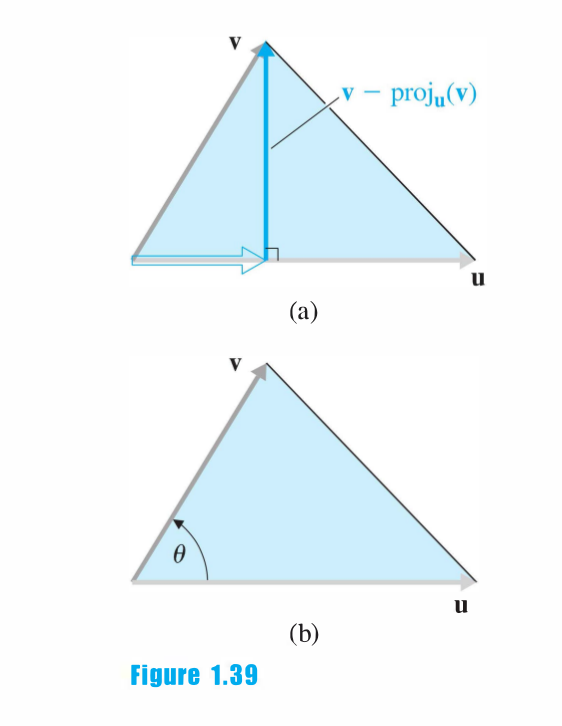
\includegraphics[scale=.25]{fig139}
\end{minipage}
\\
 \\
Exercise 46: \\
\[ A = (1, -1), B = (2,2), C = (4, 0)\]
\end{problem}


% End of problem

\pagebreak

\begin{problem}
\textbf{60:}  Suppose we know that $\vec{u} \cdot \vec{ v} = \vec{u} \cdot \vec{w}$. Does it follow that
$\vec{v} = \vec{w}$? If it does, give a proof that is valid in $\mathbb{R}^n$;
otherwise, give a counterexample (i.e., a specific set of
vectors $\vec{u}$, $\vec{v}$, and $\vec{w}$ for which $\vec{u} \cdot \vec{v} = \vec{u}\cdot \vec{w}$ but $\vec{v} \ne \vec{w}$).
\end{problem}


\vspace{180pt}
\pagebreak
% End of problem

\begin{problem}
\textbf{62:}\\
\textbf{(a) }  Prove that \[ \|\vec{u} + \vec{v}\|^2 + \|\vec{u} - \vec{v}\|^2 = 2\|\vec{u}\|^2 + 2\|\vec{v}\|^2 \]
for all vectors $\vec{u}$ and $\vec{v}$ in $\mathbb{R} ^n$. \\
\textbf{(b) } Draw a diagram showing $\vec{u}, \vec{v}, \vec{u} + \vec{v}, \text{and} \vec{u} - \vec{v}$
in $\mathbb{R}^2$ and use (a) to deduce a result about
parallelograms.
\end{problem}


% End of problem
\pagebreak

\begin{problem}
\textbf{68b:}\\
Prove that if $\vec{u}$ is orthogonal to both $\vec{v}$ and $\vec{w}$, then
$\vec{u}$ is orthogonal to s$\vec{v}$ + t$\vec{w}$ for all scalars s and t.
\end{problem}


% End of problem

\pagebreak
\section{Section 1.3}

\begin{problem}
\textbf{6:} \textit{$^*$In Exercises 3-6, write the equation of the line passing
through P with direction vector $\vec{d}$ in (a) vector form and
(b) parametric form.} \\
\[ P = (3,0,-2), \vec{d} = \begin{bmatrix} 2\\5\\0 \end{bmatrix} \]
\end{problem}



\vspace{180pt}
\pagebreak
% End of problem

\begin{problem}
\textbf{10:} \textit{$^*$In Exercises 9 and 1 0, write the equation of the plane passing
through P with direction vectors $\vec{u}$ and $\vec{v}$ in (a) vector
form and (b) parametric form.} \\
\[ P = (6,-4,-3), \vec{u} = \begin{bmatrix} 0\\1\\1 \end{bmatrix}, \vec{v} = \begin{bmatrix} -1\\1\\1 \end{bmatrix} \]
\end{problem}


% End of problem

\pagebreak

\begin{problem}
\textbf{16ace:}\\
Consider the vector equation \[\vec{x} = \vec{p} + t(\vec{q} - \vec{p})\]where
$\vec{p}$ and $\vec{q}$ correspond to distinct points P and Q in $\mathbb{R}^2$ or $\mathbb{R}^3$ \\
\textbf{(a)} Show that this equation describes the line segment $\vec{PQ}$ as t varies from 0 to 1. \\
\textbf{(c)} Find the midpoint of $\vec{PQ}$ when P = (2, - 3) and Q = (0, 1).  \\
\textbf{(e)} Find the two points that divide $\vec{PQ}$ in part (c) into three equal parts. \\
\end{problem}


\vspace{180pt}
\pagebreak
% End of problem

\begin{problem}
\textbf{18:}\\
The line $\ell$ passes through the point \textit{P} = ( 1, - 1, 1) and
has direction vector $\vec{d} = \begin{matrix}2\\3\\-1\end{matrix}$.\\ For each of the following planes $\mathcal{P}$ determine whether $\ell$ and  $\mathcal{P}$ are parallel, perpendicular, or neither:  \\
\textbf{(a)} $ 2x + 3y  - z = 1$ \\
\textbf{(b)} $ 4x - y + 5z = 0$ \\
\textbf{(c)} $ x - y -z = 3$ \\
\textbf{(d)} $ 4x + 6y - 2z = 0$ \\
\end{problem}


%End of problem

\pagebreak

\begin{problem}
\textbf{46:} \textit{$^*$In Exercises 45-46, show that the plane and line with the
given equations intersect, and then find the acute angle of
intersection between them.}\\
The plane given by 4x - y - z = 6 and the line
given by:
\begin{equation}
\begin{split}
 x &= t \\
y &= 1 + 2t\\
z &= 2 + 3t\\
\end{split}
\end{equation}
\end{problem}


%End of problem

\pagebreak
\section{Page 49}

\begin{problem}
\textbf{4:} Use the cross product to help find the normal form of the equation of the plane.\\
\textbf{(a)} The plane passing through $P = (0, -1, 1)$, parallel to $\vec{u} = \begin{bmatrix} 0 \\ 1 \\ 1 \end{bmatrix} $ and $ \vec{v} = \begin{bmatrix} 3 \\ -1 \\ 2 \end{bmatrix} $\\
\textbf{(b)} The plane passing through $P = (0, -1, 1), Q = (2, 0, 2)$, and $R = (1, 2, -1)$ 

\end{problem}


%End of problem

\pagebreak
\section{Section 2.1}

\begin{problem}
\textbf{34:}  \textit{$^*$For Exercises 33-38, solve the linear systems in the given
exercises.}\\
Exercise 28:
\begin{equation}
\begin{split}
2x_1 + 3x_2 - x_3 &= 1\\
x_1\  \ \qquad\ + x_3 &= 0 \\
-x_1 + 2x_2 - 2x_3 &= 0
\end{split}
\end{equation}

\end{problem}


\vspace{180pt}
\pagebreak
%End of problem

\begin{problem}
\textbf{42:}  \textit{$^*$In Exercises 4 1 -44, the systems of equations are nonlinear.
Find substitutions (changes of variables) that convert each
system into a linear system and use this linear system to help
solve the given system.}\\
Exercise 28:
\begin{equation}
\begin{split}
x^2 + 2y^2 &= 6 \\
x^2 - y^2 &= 3
\end{split}
\end{equation}

\end{problem}

\end{document}